% !TeX spellcheck = en_US
\section{Semiconductors}
\paragraph{Intrinsic} semiconductor: ideal, perfect crystal without impurities.
\paragraph{Extrinsic} semiconductor: Impurities to give excess electrons or holes.

e.g. Si, Ge, GaAs, InP, \ldots

\subsection{Conduction in semiconductors}
A uniform electric field $E_x$ is applied, which leads to a linearly decreasing potential
\begin{equation}
    \frac{dV}{dx} = -E_x
\end{equation}

%TODO: add graphic

This leads to a current density of
\begin{equation}
    J = e n v_{de} + e p v_{dh}
\end{equation}
where the drift velocities and mobilities for electrons and holes are
\begin{align*}
    v_{de} &= \mu_e E_x & \mu_e &= \frac{e \tau_e}{m_e^*} \\
    v_{dh} &= \mu_h E_x & \mu_h &= \frac{e \tau_h}{m_h^*}
\end{align*}
This leads to the conductivity
\begin{equation}
    \sigma = e n \mu_e + e p \mu_h
\end{equation}

\subsection{Electron and hole concentrations}
\begin{figure}[ht!]
    \centering
    %TODO: draw pic in tikz
    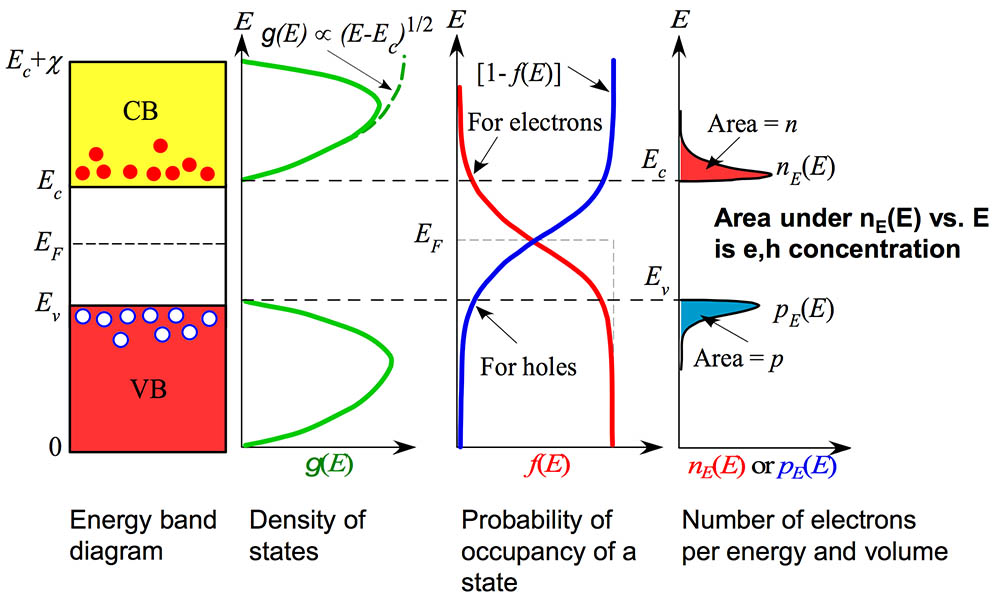
\includegraphics[width=0.6\linewidth]{images/semicond_elec_hole_concentration.jpg}
\end{figure}

The electron concentration $n$ and the hole concentration $p$ are calculated by
\begin{align}
    n &= N_C \cdot e^{-\frac{E_C-E_F}{k T}} && \text{with} & N_C &= 2 \left( \frac{2 \pi m_e^* k T}{h^2} \right)^{3/2} \\
    p &= N_V \cdot e^{-\frac{E_C-E_F}{k T}} && \text{with} & N_V &= 2 \left( \frac{2 \pi m_h^* k T}{h^2} \right)^{3/2}
\end{align}
where $N_C$ and $N_V$ are the effective densities of states at the CB edge and at the VB edge.

The \emph{mass action law} states that
\begin{equation}
    n p = n_i^2 = N_C N_V \cdot e^{-\frac{E_C-E_V}{k T}} = N_C N_V \cdot e^{-\frac{E_G}{k T}}
\end{equation}
where $n_i$ is the electron and hole concentration in an intrinsic semiconductor.

\begin{table}[hbp!]
    \centering
    \begin{tabular}{lll}
        $n = p$ & $\Rightarrow$ & intrinsic semiconductor \\
        $n > p$ & $\Rightarrow$ & n-type semiconductor \\
        $p > n$ & $\Rightarrow$ & p-type semiconductor \\
    \end{tabular}
\end{table}

The Fermi energy in an intrinsic semiconductor is
\begin{align}
    E_{Fi} &= E_V + \frac{1}{2} E_g - \frac{1}{2} k T \ln \frac{N_C}{N_V} \\
    &= E_V + \frac{1}{2} E_g - \frac{3}{4} k T \ln \frac{m_e^*}{m_h^*} \\
    &= E_V + \frac{1}{2} E_g \qquad \text{if} \quad m_e^*=m_h^* \:,\: N_C = N_V
\end{align}

The Fermi level is almost in the middle of the energy gap.
In Si and Ge, it is slightly below midgap.
%TODO: add image from 5.14


As $np = n_i^2$ must always be fulfilled,
\begin{align*}
    n \uparrow \;\Leftrightarrow\; E_F \uparrow && p \uparrow \;\Leftrightarrow\; E_F \downarrow
\end{align*}

The average energy of an electron in the conduction band is
\begin{equation}
    \bar{E}_{CB} = E_C + \frac{3}{2} kT
\end{equation}

\begin{figure}[htbp]
    \centering
    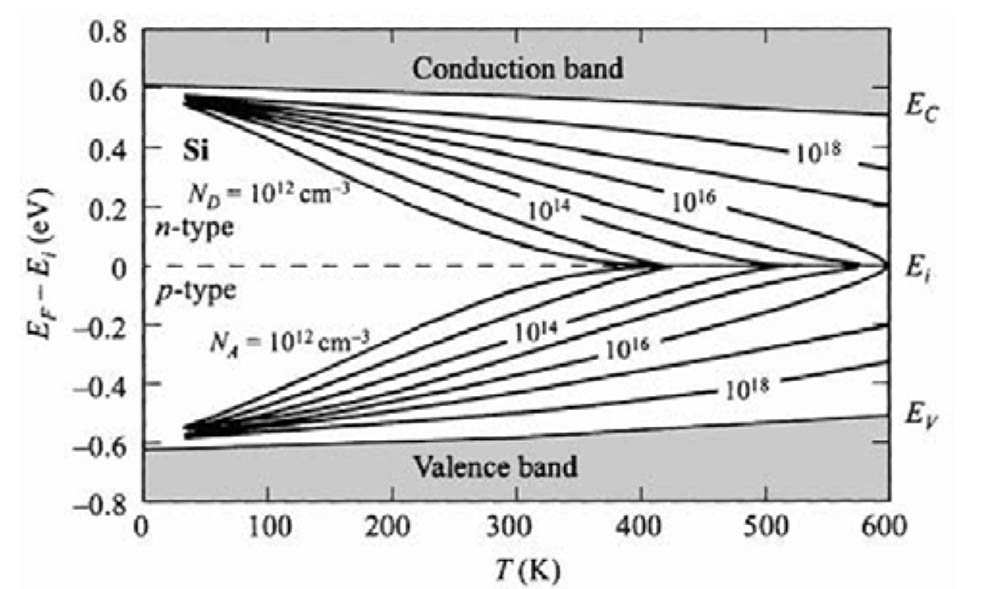
\includegraphics[width=0.6\linewidth]{images/semiconductors_fermi_energies.jpg}
    \caption{Fermi energy in silicon as a function of temperature and impurity concentration}
\end{figure}

The typical properties of some semiconductors is depicted in appendix~\ref{app:semiconductors}.

\subsection{Extrinsic semiconductors}
%TODO: bänder mit As und B einfügen, sowie formel verstehen + einfügen!--> kasap?
\paragraph{N-Type}
In n-type semiconductors, the impurity is a \emph{donor} atom, such as As, P, Sb.
This leads to an unbonded $e^-$ which orbits around the ionic center.
With $n \approx N_d$ (as $N_d \gg n_i$) this leads to
\begin{equation}
    \sigma \approx e N_d \mu_e
\end{equation}

\paragraph{P-Type}
In p-type semiconductors, the impurity is a \emph{acceptor} atom, such as B, Al, Ga, In.
This leads to a missing $e^-$ (hole) which orbits the negative site.
With $p \approx N_a$ (as $N_a \gg n_i$), this leads to
\begin{equation}
    \sigma \approx e N_a \mu_h
\end{equation}

\paragraph{Compensation doping}
is the situation in which a semiconductor contains both donors and acceptors.
Recombination takes place until either 
$n=N_d-N_a$ or $p=N_a-N_d$. 

\begin{align*}
    \text{More donors than acceptors:} && N_d - N_a &\gg n_i & n &= N_d - N_a & p &= \frac{n_i^2}{N_d-N_a} \\
    \text{More acceptors than donors:} && N_a - N_d &\gg n_i & n &= \frac{n_i^2}{N_a - N_d} & p &= N_a - N_d
\end{align*}

\subsection{Temperature dependence of conductivity}
The conductivity $\sigma = q n \mu $ where $n$ and $\mu$ are temperature dependant.

\begin{multicols}{3}
    \paragraph{Intrinsic range}
    $T > T_i$
    \begin{equation*}
        n = n_i \,\propto\, e^{\frac{E_g}{2kT}}
    \end{equation*}
    Intrinsic behavior \\
    Ionization across bandgap.
\vfill\columnbreak
    \paragraph{Extrinsic range}
    $T_s < T < T_i$
    \begin{equation*}
        n = N_d = \text{const.}
    \end{equation*}
    All donors ionized \\
    Electron conc. = donor conc.
\vfill\columnbreak    
    \paragraph{Ionization range}
    $T < T_s$
    \begin{equation*}
        n \,\propto\, e^{-\frac{\Delta E}{2kT}}
    \end{equation*}
    Donor ionization\\
     $T_s$: Saturation temperature.
\vfill
\end{multicols}

%TODO insert image from slide 21-23

\paragraph{Intrinsic carrier concentration}
The temperature dependence comes from the mass action law.
The slope is a measure of energy gap.
\begin{equation}
    n_i = \sqrt{np} = \sqrt{N_C N_V} e^{\frac{E_g}{2kT}}
\end{equation}

\paragraph{Drift mobility}

\subsection{Direct and indirect recombination}

\subsection{Optical absorption}

\subsection{Schottky junction}

\subsection{Ohmic contact}